\documentclass[12pt,a4paper]{article}

% ---- Ngôn ngữ & Font ----
\usepackage{fontspec}
\usepackage[vietnamese]{babel} 
\setmainfont{Times New Roman}  
\setmonofont{Courier New}[Scale=0.90]


% ---- Trang giấy ----
\usepackage[margin=2.5cm,top=2.5cm,bottom=2.5cm]{geometry}
\usepackage{setspace}
\onehalfspacing

% ---- Toán học ----
\usepackage{amsmath, amssymb, amsthm, mathtools}

% ---- Bảng biểu ----
\usepackage{booktabs}
\usepackage{array}
\usepackage{longtable}
\usepackage{tabularx}
\usepackage{multirow}
\usepackage{ragged2e}
\newcolumntype{C}[1]{>{\centering\arraybackslash}m{#1}}
\newcolumntype{R}[1]{>{\raggedleft\arraybackslash}m{#1}}
\newcolumntype{L}[1]{>{\raggedright\arraybackslash}m{#1}}

% ---- Hình ảnh & Màu ----
\usepackage{graphicx}
\usepackage{float}
\usepackage{xcolor}
\usepackage{pifont}

\newcommand{\okmark}{\textcolor{green!55!black}{\ding{51}}}
\newcommand{\warnmark}{\textcolor{orange!90!black}{\ding{115}}}
\newcommand{\nokmark}{\textcolor{red!80!black}{\ding{55}}}

% ---- Hyperlink & Mục lục ----
\usepackage[hidelinks]{hyperref}
\hypersetup{colorlinks=true, linkcolor=black, urlcolor=blue!70!black, citecolor=blue!70!black}

% ---- Sơ đồ TikZ ----
\usepackage{tikz}
\usetikzlibrary{shapes.geometric, arrows.meta, positioning, fit, backgrounds, calc}

% ---- Code listing ----
\usepackage{listings}
\definecolor{codegreen}{rgb}{0.00,0.55,0.00}
\definecolor{codegray}{rgb}{0.50,0.50,0.50}
\definecolor{codepurple}{rgb}{0.58,0.00,0.82}
\definecolor{codeblue}{rgb}{0.13,0.29,0.53}
\definecolor{backcolour}{rgb}{0.97,0.97,0.95}

\lstdefinestyle{pythonstyle}{
  backgroundcolor=\color{backcolour},
  commentstyle=\color{codegreen}\itshape,
  keywordstyle=\color{codeblue}\bfseries,
  numberstyle=\tiny\color{codegray},
  stringstyle=\color{codepurple},
  basicstyle=\ttfamily\footnotesize,
  breakatwhitespace=false,
  breaklines=true,
  captionpos=b,
  keepspaces=true,
  numbers=left,
  numbersep=6pt,
  showspaces=false,
  showstringspaces=false,
  showtabs=false,
  tabsize=2,
  language=Python,
  extendedchars=true,
  upquote=true,
  frame=single,
  framesep=4pt,
  xleftmargin=10pt
}
\lstset{style=pythonstyle}

% ---- Đầu trang / Chân trang ----
\usepackage{fancyhdr}
\pagestyle{fancy}
\fancyhf{}
\fancyhead[L]{\small\itshape Đồ án 2 — Data Fitting và Phương Pháp OLS}
\fancyhead[R]{\small\itshape Nhóm 03}
\fancyfoot[C]{\thepage}
\renewcommand{\headrulewidth}{0.3pt}

% ---- Tiêu đề mục ----
\usepackage{titlesec}
\renewcommand{\thesection}{\Roman{section}}
\renewcommand{\thesubsection}{\arabic{subsection}}
\titleformat{\section}{\Large\bfseries}{\thesection.}{0.5em}{}
\titleformat{\subsection}{\large\bfseries}{\thesubsection.}{0.5em}{}
\titleformat{\subsubsection}{\normalsize\bfseries}{\thesubsubsection.}{0.5em}{}

% =========================================================================
\begin{document}

% =================================================================
% ===================== TRANG 1: BÌA ==============================
% =================================================================
\begin{titlepage}
    \begin{tikzpicture}[overlay, remember picture]
        \def\margin{0.8cm} \def\gap{0.2cm}
        \draw[line width=1.5pt] ($ (current page.north west) + (\margin, -\margin) $) rectangle ($ (current page.south east) + (-\margin, \margin) $);
        \draw[line width=0.5pt] ($ (current page.north west) + (\margin+\gap, -\margin-\gap) $) rectangle ($ (current page.south east) + (-\margin-\gap, \margin+\gap) $);
    \end{tikzpicture}
    
    \begin{center}
        {\fontsize{13pt}{15pt}\selectfont \textbf{ĐẠI HỌC QUỐC GIA THÀNH PHỐ HỒ CHÍ MINH\\ TRƯỜNG ĐẠI HỌC KHOA HỌC TỰ NHIÊN\\ KHOA CÔNG NGHỆ THÔNG TIN}}

        \vfill
        
\includegraphics[width=4cm]{images/logo.png}
        \vfill
        
        {\fontsize{20pt}{22pt}\selectfont \textbf{ĐỒ ÁN 2}} \\
        \vspace{0.5cm}
        {\fontsize{16pt}{20pt}\selectfont \textbf{DATA FITTING VÀ PHƯƠNG PHÁP OLS\\ ỨNG DỤNG DỰ ĐOÁN HUYẾT ÁP TÂM THU}} \\
        
        \vfill
        \begin{tabular}{rl}
            \textbf{Môn học:} & Toán Ứng Dụng \& Thống Kê \\
            \textbf{Mã môn:} & MTH00051 \\
            \textbf{Học kỳ:} & Học kỳ 2, 2025-2026 \\
        \end{tabular}

        \vspace{1.0cm}
        \begin{tabular}{rl}
            \textbf{Giảng viên hướng dẫn:} & ThS. Võ Nam Thục Đoan, ThS. Lê Nhựt Nam \\
            \textbf{Nhóm thực hiện:} & 03 \\ 
        \end{tabular}

        \vfill
        \textbf{Thành viên thực hiện:} \\
        \vspace{0.5cm}
        \begin{tabular}{|l|l|}
            \hline
            \textbf{Mã số sinh viên} & \textbf{Họ và tên} \\
            \hline
            24120072 & Lê Công Anh Khoa \\
            \hline
            24120242 & Lê Ngọc Tuyền \\
            \hline
            24120253 & Đặng Quốc An \\
            \hline
            24120334 & Hoàng Khang \\
            \hline
            24120372 & Nguyễn Hữu Hoàng Long \\
            \hline
        \end{tabular}
        \vfill
        {\fontsize{14pt}{20pt}\selectfont \textbf{THÀNH PHỐ HỒ CHÍ MINH, 2026}}
    \end{center}
\end{titlepage}

% =================================================================
% ================ TRANG 2: PHÂN CÔNG CÔNG VIỆC ===================
% =================================================================
\newpage
\pagestyle{empty}
\begin{center}
{\LARGE\bfseries BẢNG PHÂN CÔNG CÔNG VIỆC}
\end{center}
\vspace{1.0cm}

\renewcommand{\arraystretch}{2.2}
\begin{center}
\begin{tabular}{|C{2.2cm}|C{4.2cm}|C{5.2cm}|C{2.6cm}|}
\hline
\textbf{Mã số sinh viên} & \textbf{Họ tên} & \textbf{Phân công} & \textbf{Tỷ lệ hoàn thành} \\ \hline
24120372 & Nguyễn Hữu Hoàng Long & Lý thuyết \& Cài đặt OLS, Inference & 100\%\\ \hline
24120253 & Đặng Quốc An & Cài đặt Ridge/Lasso, VIF \& Cross-Validation & 100\%\\ \hline
24120242 & Lê Ngọc Tuyền  & EDA \& Data Pipeline (Xử lý missing values) & 100\% \\ \hline
24120072 & Lê Công Anh Khoa & Xây dựng, huấn luyện \& So sánh 3 mô hình & 100\% \\ \hline
24120334 & Hoàng Khang & Phân tích phần dư, Kết luận y khoa \& Tổng hợp báo cáo & 100\% \\ \hline
\end{tabular}
\end{center}
\renewcommand{\arraystretch}{1.0}

% =================================================================
% ===================== TRANG 3: MỤC LỤC ==========================
% =================================================================
\newpage
\pagestyle{fancy}
\setcounter{page}{1}
\renewcommand{\contentsname}{\centerline{MỤC LỤC}}
\tableofcontents
\newpage

% =================================================================
% =================== NỘI DUNG CHÍNH ==============================
% =================================================================

\section{Lý thuyết data fitting và OLS}

\subsection{Bài toán Data Fitting và mô hình tuyến tính}
% Nội dung từ 1.1
Bài toán Data Fitting là tìm một hàm $f : \mathbb{R}^p \to \mathbb{R}$ xấp xỉ tốt nhất mối quan hệ giữa các biến độc lập $\mathbf{x}_i \in \mathbb{R}^p$ và biến phụ thuộc $y_i \in \mathbb{R}$ từ tập dữ liệu quan sát $\mathcal{D} = \{(\mathbf{x}_i, y_i)\}_{i=1}^{n}$. Trong mô hình hồi quy tuyến tính đa biến, ta giả sử mối quan hệ này có dạng:
\begin{equation}
y_i = \beta_0 + \beta_1 x_{i1} + \dots + \beta_p x_{ip} + \varepsilon_i = \mathbf{x}_i^T \boldsymbol{\beta} + \varepsilon_i
\end{equation}
với $\boldsymbol{\beta} = (\beta_0, \beta_1, \dots, \beta_p)^T$ là vector tham số cần ước lượng và $\varepsilon_i$ là nhiễu ngẫu nhiên. Biểu diễn dưới dạng ma trận:
\begin{equation}
\mathbf{y} = \mathbf{X}\boldsymbol{\beta} + \boldsymbol{\varepsilon}
\end{equation}
trong đó $\mathbf{X} \in \mathbb{R}^{n \times (p+1)}$ là ma trận thiết kế với cột đầu tiên là vector $\mathbf{1}$ đại diện cho hệ số chặn.

\subsection{Giả thiết Gauss–Markov (GM1–GM5)}
Các giả thiết cơ bản (Gauss-Markov) để đảm bảo tính hợp lệ của mô hình OLS bao gồm:
\begin{itemize}
    \item \textbf{GM1 (Tuyến tính):} Mô hình có dạng tuyến tính $\mathbf{y} = \mathbf{X}\boldsymbol{\beta} + \boldsymbol{\varepsilon}$.
    \item \textbf{GM2 (Không đa cộng tuyến hoàn hảo):} Ma trận $\mathbf{X}$ có hạng cột đầy đủ, $\text{rank}(\mathbf{X}) = p + 1$.
    \item \textbf{GM3 (Ngoại sinh):} Kỳ vọng có điều kiện của phần dư bằng 0, $\mathbb{E}[\boldsymbol{\varepsilon} \mid \mathbf{X}] = \mathbf{0}$.
    \item \textbf{GM4 (Đồng phương sai):} Phương sai của sai số không đổi và các sai số không có tương quan, $\text{Var}(\boldsymbol{\varepsilon} \mid \mathbf{X}) = \sigma^2 \mathbf{I}_n$.
    \item \textbf{GM5 (Phân phối chuẩn):} Nhiễu tuân theo phân phối chuẩn $\boldsymbol{\varepsilon} \mid \mathbf{X} \sim \mathcal{N}(\mathbf{0}, \sigma^2 \mathbf{I}_n)$.
\end{itemize}

\subsection{Ước lượng bình phương bé nhất và ma trận hình mũ}
Ước lượng OLS tìm vector $\hat{\boldsymbol{\beta}}$ nhằm cực tiểu hóa tổng bình phương phần dư (RSS):
\begin{equation}
\text{RSS}(\boldsymbol{\beta}) = \|\mathbf{y} - \mathbf{X}\boldsymbol{\beta}\|_2^2 = (\mathbf{y} - \mathbf{X}\boldsymbol{\beta})^T(\mathbf{y} - \mathbf{X}\boldsymbol{\beta})
\end{equation}
Chứng minh: Tính đạo hàm của hàm $\text{RSS}$ theo $\boldsymbol{\beta}$ và cho bằng $\mathbf{0}$:
\begin{equation}
\frac{\partial \text{RSS}}{\partial \boldsymbol{\beta}} = -2\mathbf{X}^T\mathbf{y} + 2\mathbf{X}^T\mathbf{X}\boldsymbol{\beta} = \mathbf{0} \implies \mathbf{X}^T\mathbf{X}\boldsymbol{\beta} = \mathbf{X}^T\mathbf{y}
\end{equation}
Do giả thiết GM2, $\mathbf{X}^T\mathbf{X}$ khả nghịch, ta thu được nghiệm dạng đóng:
\begin{equation}
\hat{\boldsymbol{\beta}} = (\mathbf{X}^T\mathbf{X})^{-1}\mathbf{X}^T\mathbf{y}
\end{equation}

Ma trận chiếu ($\mathbf{H}$): Là ma trận chiếu $\mathbf{y}$ lên không gian cột của $\mathbf{X}$ để tạo ra giá trị dự đoán $\hat{\mathbf{y}} = \mathbf{H}\mathbf{y}$, định nghĩa bởi:
\begin{equation}
\mathbf{H} = \mathbf{X}(\mathbf{X}^T\mathbf{X})^{-1}\mathbf{X}^T
\end{equation}
Ma trận này có các tính chất quan trọng: đối xứng ($\mathbf{H}^T = \mathbf{H}$) và lũy đẳng ($\mathbf{H}^2 = \mathbf{H}$).

\subsection{Định lý Gauss–Markov và thực nghiệm mô phỏng Monte Carlo}
Định lý Gauss-Markov phát biểu rằng: Dưới các giả thiết GM1 đến GM4, $\hat{\boldsymbol{\beta}}_{OLS}$ là ước lượng tuyến tính không chệch tốt nhất (BLUE).
\begin{itemize}
    \item \textbf{Tuyến tính:} $\hat{\boldsymbol{\beta}}$ là tổ hợp tuyến tính của $\mathbf{y}$.
    \item \textbf{Không chệch:} $\mathbb{E}[\hat{\boldsymbol{\beta}}] = \boldsymbol{\beta}$.
    \item \textbf{Tốt nhất:} Trong tất cả các ước lượng tuyến tính không chệch, OLS có ma trận hiệp phương sai nhỏ nhất (theo nghĩa ma trận bán xác định dương): $\text{Var}(\hat{\boldsymbol{\beta}}_{OLS}) = \sigma^2(\mathbf{X}^T\mathbf{X})^{-1}$.
\end{itemize}

Thông qua mô phỏng Monte Carlo (lặp lại việc sinh dữ liệu nhiễu và ước lượng hệ số hàng nghìn lần), trung bình của các ước lượng hội tụ chính xác về $\boldsymbol{\beta}$ thực tế. Khi so sánh với các ước lượng tuyến tính không chệch khác (được làm nhiễu có chủ ý), phân phối của OLS luôn có phương sai nhỏ (đồ thị hẹp hơn), minh chứng thực tế cho tính chất BLUE.

\begin{figure}[H]
\centering

\includegraphics[width=0.65\textwidth]{images/fig_gauss_markov.png}
\caption{Minh họa định lý Gauss-Markov qua mô phỏng Monte Carlo.}
\label{fig:gauss_markov}
\end{figure}

\subsection{Đánh giá độ tương hợp của mô hình và kiểm định ý nghĩa tổng thể}
Để đánh giá độ phù hợp của mô hình với dữ liệu, ta dùng hệ số xác định $R^2$:
\begin{equation}
R^2 = 1 - \frac{\text{RSS}}{\text{TSS}} = 1 - \frac{\sum (y_i - \hat{y}_i)^2}{\sum (y_i - \bar{y})^2}
\end{equation}
Để tránh việc $R^2$ luôn tăng khi thêm biến vô nghĩa, hệ số $R^2$ hiệu chỉnh ($\bar{R}^2$) phạt số lượng biến $p$:
\begin{equation}
\bar{R}^2 = 1 - \left(1 - R^2\right) \frac{n - 1}{n - p - 1}
\end{equation}
Kiểm định F: Đánh giá ý nghĩa tổng thể của mô hình. Giả thuyết $H_0: \beta_1 = \dots = \beta_p = 0$. Thống kê kiểm định:
\begin{equation}
F = \frac{(\text{TSS} - \text{RSS})/p}{\text{RSS}/(n - p - 1)} \sim F_{(p, n-p-1)}
\end{equation}

\subsection{Kiểm định ý nghĩa thống kê của các hệ số hồi quy}
Để kiểm định ý nghĩa của từng hệ số $\beta_j$, ta dùng kiểm định t với giả thuyết $H_0: \beta_j = 0$. Thống kê t:
\begin{equation}
t_j = \frac{\hat{\beta}_j}{\text{SE}(\hat{\beta}_j)} = \frac{\hat{\beta}_j}{\hat{\sigma}\sqrt{[(\mathbf{X}^T\mathbf{X})^{-1}]_{jj}}} \sim t_{(n-p-1)}
\end{equation}
Khoảng tin cậy $95\%$ cho $\beta_j$ được tính bởi:
\begin{equation}
\text{CI} = \hat{\beta}_j \pm t_{\alpha/2} \cdot \text{SE}(\hat{\beta}_j)
\end{equation}

\begin{figure}[H]
\centering

\includegraphics[width=0.65\textwidth]{images/fig_confidence_intervals.png}
\caption{Khoảng tin cậy 95\% cho từng hệ số hồi quy.}
\label{fig:ci}
\end{figure}

\newpage
\subsection{Hiện tượng đa cộng tuyến và hệ số phóng đại phương sai}
Đa cộng tuyến xảy ra khi các biến độc lập có sự tương quan tuyến tính mạnh với nhau, làm ma trận $\mathbf{X}^T\mathbf{X}$ gần suy biến và thổi phồng phương sai của hệ số $\hat{\boldsymbol{\beta}}$.
Định lượng bằng hệ số phóng đại phương sai (VIF):
\begin{equation}
\text{VIF}_j = \frac{1}{1 - R_j^2}
\end{equation}
trong đó $R_j^2$ là hệ số $R^2$ khi hồi quy biến $X_j$ lên tất cả các biến $X$ còn lại. Nếu $\text{VIF}_j > 10$, biến $X_j$ có hiện tượng đa cộng tuyến nghiêm trọng và cần được xử lý (như loại bỏ biến hoặc dùng điều chuẩn).

\begin{figure}[H]
\centering

\includegraphics[width=0.65\textwidth]{images/fig_vif.png}
\caption{Đánh giá Đa cộng tuyến thông qua biểu đồ VIF.}
\label{fig:vif}
\end{figure}

\subsection{Điều chuẩn: Ridge, Lasso, Ridge trace}
Để khắc phục đa cộng tuyến hoặc overfitting, ta thêm các thành phần điều chuẩn vào hàm mất mát.

Hồi quy Ridge (phạt $L_2$):
\begin{equation}
\hat{\boldsymbol{\beta}}_{\text{Ridge}} = \arg\min_{\boldsymbol{\beta}} \left\{ \|\mathbf{y} - \mathbf{X}\boldsymbol{\beta}\|_2^2 + \lambda\|\boldsymbol{\beta}\|_2^2 \right\} = (\mathbf{X}^T\mathbf{X} + \lambda\mathbf{I})^{-1}\mathbf{X}^T\mathbf{y}
\end{equation}
Nghiệm Ridge là dạng đóng và luôn khả nghịch nhờ đường chéo $\lambda\mathbf{I}$.

Hồi quy Lasso (phạt $L_1$):
\begin{equation}
\hat{\boldsymbol{\beta}}_{\text{Lasso}} = \arg\min_{\boldsymbol{\beta}} \left\{ \|\mathbf{y} - \mathbf{X}\boldsymbol{\beta}\|_2^2 + \lambda\|\boldsymbol{\beta}\|_1 \right\}
\end{equation}
Lasso không có nghiệm dạng đóng, do đó được giải bằng các thuật toán lặp như hạ gradient tọa độ. Lasso có khả năng thu gọn một số hệ số về đúng $0$, hoạt động như lựa chọn đặc trưng tự nhiên.

\begin{figure}[H]
\centering

\includegraphics[width=0.65\textwidth]{images/fig_ridge_trace.png}
\caption{Ridge Trace: Sự thay đổi của hệ số theo tham số phạt $\lambda$.}
\label{fig:ridge_trace}
\end{figure}

\subsection{Đánh giá giả thuyết mô hình qua phân tích phần dư}
Phân tích phần dư ($\hat{\boldsymbol{\varepsilon}} = \mathbf{y} - \hat{\mathbf{y}}$) giúp đánh giá lại các giả thiết Gauss-Markov. Biểu đồ Residuals vs Fitted cho thấy các điểm phân tán ngẫu nhiên quanh $0$, giúp kiểm tra tính tuyến tính của mô hình. Biểu đồ Normal Q-Q giúp đánh giá phân phối chuẩn của phần dư, trong khi Scale-Location dùng để kiểm tra giả thiết đồng phương sai. Cuối cùng, Residuals vs Leverage hỗ trợ phát hiện các điểm dữ liệu có ảnh hưởng quá lớn làm lệch mô hình.

\begin{figure}[H]
\centering

\includegraphics[width=0.75\textwidth]{images/fig_residual_plots.png}
\caption{Bốn biểu đồ chẩn đoán phần dư chuẩn của mô hình hồi quy tuyến tính.}
\label{fig:residuals}
\end{figure}

\newpage
\subsection{Kiểm chứng chéo: K-Fold CV, CV score}
Kiểm chứng chéo K-Fold là phương pháp chia dữ liệu ngẫu nhiên thành $k$ phần. Mỗi lần lặp, mô hình dùng $k-1$ phần huấn luyện và $1$ phần còn lại để kiểm thử. Quá trình lặp $k$ lần, tính trung bình lỗi (MSE):
\begin{equation}
\text{CV}_{(k)} = \frac{1}{k} \sum_{i=1}^{k} \text{MSE}_i
\end{equation}
Phương pháp này giúp đánh giá độ tổng quát hóa của mô hình và thường được dùng để chọn siêu tham số tối ưu (như $\lambda$).

\begin{figure}[H]
\centering

\includegraphics[width=0.65\textwidth]{images/fig_cv_lambda.png}
\caption{Lựa chọn tham số $\lambda$ tối ưu cho mô hình Ridge thông qua k-Fold CV.}
\label{fig:cv_lambda}
\end{figure}

% =================================================================
% =================== NỘI DUNG CHÍNH: PHẦN 2 ======================
% =================================================================
\newpage
\section{Ứng dụng: Dự đoán huyết áp tâm thu}
 
\subsection{Tổng quan về bộ dữ liệu y khoa NHANES}
Bộ dữ liệu Khảo sát Khám sức khỏe và Dinh dưỡng Quốc gia Hoa Kỳ (NHANES) chu kỳ 2021–2023 được thu thập bởi CDC \cite{nhanes2023}, bao gồm các chỉ số nhân khẩu học, nhân trắc học và sinh hóa máu trên mẫu đại diện dân số Hoa Kỳ. Mục tiêu của Phần 2 là xây dựng và đánh giá các mô hình hồi quy dự đoán huyết áp tâm thu (SBP) — chỉ số trực tiếp dùng để chẩn đoán tăng huyết áp và sàng lọc nguy cơ đột quỵ, nhồi máu cơ tim. Nghiên cứu thực hiện liên kết 10 học phần dữ liệu thô thông qua mã định danh người tham gia \texttt{SEQN}, lấy học phần nhân khẩu học làm bảng gốc như mô tả trong Bảng \ref{tab:nhanes_modules}.

\begin{table}[H]
\centering
\caption{Mô tả các học phần dữ liệu thô trích xuất từ NHANES 2021–2023}
\label{tab:nhanes_modules}
\small
\begin{tabular}{lll}
\toprule
\textbf{Tên file SAS} & \textbf{Học phần nội dung} & \textbf{Các biến đặc trưng tiêu biểu} \\
\midrule
\texttt{DEMO\_L.xpt} & Nhân khẩu học & \texttt{RIDAGEYR} (Tuổi), \texttt{RIAGENDR} (Giới tính) \\
\texttt{BPXO\_L.xpt} & Đo huyết áp & \texttt{BPXOSY1/2/3} (Tâm thu), \texttt{BPXOPLS1/2/3} (Nhịp tim) \\
\texttt{BMX\_L.xpt} & Đo nhân trắc học & \texttt{BMXHT} (Chiều cao), \texttt{BMXWT} (Cân nặng), \texttt{BMXBMI} (BMI) \\
\texttt{SMQ\_L.xpt} & Hành vi hút thuốc & \texttt{SMQ020} (Từng hút ít nhất 100 điếu thuốc) \\
\texttt{DIQ\_L.xpt} & Bệnh tiểu đường & \texttt{DIQ010} (Đã từng được chẩn đoán tiểu đường) \\
\texttt{TCHOL\_L.xpt} & Cholesterol toàn phần & \texttt{LBXTC} (Nồng độ Cholesterol toàn phần trong máu) \\
\texttt{BIOPRO\_L.xpt} & Sinh hóa máu & \texttt{LBXSCR} (Creatinine huyết thanh - chức năng thận) \\
\texttt{MCQ\_L.xpt} & Tiền sử bệnh lý & \texttt{MCQ160E} (Tiền sử đột quỵ), \texttt{MCQ160F} (Bệnh mạch vành) \\
\texttt{ALQ\_L.xpt} & Sử dụng rượu bia & \texttt{ALQ130} (Số ly rượu uống trung bình hàng ngày) \\
\texttt{PAQ\_L.xpt} & Hoạt động thể chất & \texttt{PAQ680} (Thời gian ngồi thụ động hàng ngày) \\
\bottomrule
\end{tabular}
\end{table}

\subsection{Phân tích khám phá dữ liệu (EDA)}
Dữ liệu thô thu được sau khi kết nối có kích thước 11,933 dòng × 21 cột. Nhằm khảo sát phân phối của các đặc trưng sinh học và phát hiện bất thường, lớp phân tích khám phá dữ liệu \texttt{EDA} trong \texttt{data\_pipeline.py} được xây dựng thủ công từ đầu. Đối với các đặc trưng liên tục, trung bình mẫu được tính bằng công thức:
\begin{equation}
\bar{x}_j = \frac{1}{n_{\text{known}}} \sum_{i \in \text{known}} x_{ij}
\end{equation}
và độ lệch chuẩn mẫu hiệu chỉnh được xác định qua:
\begin{equation}
s_j = \sqrt{\frac{1}{n_{\text{known}} - 1} \sum_{i \in \text{known}} (x_{ij} - \bar{x}_j)^2}
\end{equation}
Các phân vị Q1, Q2 và Q3 được tính bằng cách sắp xếp danh sách các quan sát thực tế tăng dần và trích xuất giá trị tại các vị trí phân vị tương ứng ($25\%$, $50\%$, $75\%$). Tỷ lệ khuyết thiếu của mỗi đặc trưng được xác định bằng tỉ số giữa số mẫu trống và tổng số mẫu trong bộ dữ liệu. 

Kết quả phân tích cho thấy bộ dữ liệu thực tế này có tỷ lệ khuyết thiếu khá cao ở một số biến sinh hóa máu, cụ thể là Cholesterol toàn phần \texttt{LBXTC} khuyết $37.8\%$ và Creatinine huyết thanh \texttt{LBXSCR} khuyết $36.5\%$ . Biến mục tiêu \texttt{SYSTOLIC\_TARGET} có phân phối tiệm cận chuẩn và lệch phải nhẹ, phản ánh thực tế dân số có xu hướng tăng huyết áp khi lớn tuổi. Các thông số mô tả của các đặc trưng liên tục được tổng hợp trong Bảng \ref{tab:eda_summary}.

\begin{table}[H]
\centering
\caption{Thống kê mô tả các đặc trưng liên tục chính trước khi chuẩn hóa}
\label{tab:eda_summary}
\small
\begin{tabular}{lcccccc}
\toprule
\textbf{Biến đặc trưng} & \textbf{Trung bình} & \textbf{Độ lệch chuẩn} & \textbf{Min} & \textbf{Q1} & \textbf{Trung vị} & \textbf{Max} \\
\midrule
\texttt{RIDAGEYR} (Tuổi) & 48.24 & 18.32 & 18.00 & 32.00 & 49.00 & 80.00 \\
\texttt{BMXBMI} (BMI) & 29.85 & 7.12 & 13.20 & 24.60 & 28.70 & 86.20 \\
\texttt{BPXOPLS} (Nhịp tim) & 71.42 & 11.85 & 36.00 & 63.33 & 70.67 & 136.00 \\
\texttt{LBXTC} (Cholesterol) & 192.45 & 41.56 & 69.00 & 163.00 & 189.00 & 422.00 \\
\texttt{LBXSCR} (Creatinine) & 0.88 & 0.35 & 0.23 & 0.71 & 0.84 & 9.85 \\
\texttt{SYSTOLIC\_TARGET} & 122.56 & 16.48 & 76.00 & 111.33 & 120.33 & 226.67 \\
\bottomrule
\end{tabular}
\end{table}

\subsection{Quy trình tiền xử lý dữ liệu và \texttt{DataPipeline}}
Quy trình tiền xử lý được chia làm hai giai đoạn tách biệt rõ ràng nhằm loại bỏ hoàn toàn hiện tượng rò rỉ dữ liệu từ tập kiểm thử sang tập huấn luyện.

Trong giai đoạn làm sạch và lọc thô bằng \texttt{prep\_checkpoint.py}, các dòng không có bất kỳ lần đo huyết áp khả dụng nào hoặc chứa giá trị phi lý về mặt sinh lý học lâm sàng được loại bỏ triệt để. Ta gộp ba lần đo đối với huyết áp tâm thu và nhịp tim bằng cách lấy trung bình cộng các lần đo khả dụng để sinh ra hai đặc trưng tương ứng là \texttt{SYSTOLIC\_TARGET} và \texttt{BPXOPLS}. Kết quả thu được tệp tin trung gian \texttt{nhanes\_pre\_pipeline.csv} gồm 7,515 dòng.

Giai đoạn hai thực hiện chuỗi biến đổi khép kín của \texttt{DataPipeline} sau khi chia dữ liệu theo tỷ lệ 80\% huấn luyện (6,012 dòng) và 20\% kiểm thử (1,503 dòng) với hạt giống ngẫu nhiên \texttt{seed=42}. Lớp \texttt{DataPipeline} được thiết kế theo chuẩn hướng đối tượng với quy trình biến đổi tuyến tính:
Đầu tiên, một kho dữ liệu mẫu hoàn chỉnh được trích xuất từ tập huấn luyện để làm tập dữ liệu gốc, sau đó được lọc các điểm dị biệt bằng phương pháp IQR. Khi gặp mẫu bị khuyết đặc trưng, thuật toán KNN Imputer tự xây dựng sẽ tính khoảng cách Euclid chuẩn hóa có trọng số nghịch đảo khoảng cách để tìm ra 5 láng giềng gần nhất, rồi điền khuyết bằng phương pháp lấy trung bình cho biến liên tục và bầu chọn số đông cho biến phân loại. Sau khi điền khuyết, các biến phân loại được mã hóa One-Hot Encoding loại bỏ cột đầu tiên để tránh đa cộng tuyến, các đặc trưng liên tục được chuẩn hóa Z-score tĩnh dựa trên các tham số học từ tập Train, và cuối cùng một cột bias toàn giá trị $1.0$ được chèn vào vị trí đầu tiên của ma trận đặc trưng.

\subsection{Xây dựng 3 mô hình (OLS full, OLS selective, Ridge)}
Các mô hình hồi quy đều sử dụng các hàm nền tảng được thiết lập từ đầu ở Phần 1, tác động lên ma trận đặc trưng $\mathbf{X} \in \mathbb{R}^{n \times 10}$ và vector nhãn $\mathbf{y} \in \mathbb{R}^n$. Mô hình đầu tiên được thử nghiệm là OLS đầy đủ sử dụng toàn bộ 9 đặc trưng thu được sau Pipeline. Nghiệm OLS được giải qua phương trình chuẩn tắc:
\begin{equation}
\hat{\boldsymbol{\beta}}_{\text{Full}} = (\mathbf{X}^T \mathbf{X})^{-1} \mathbf{X}^T \mathbf{y}
\end{equation}
Tiếp theo, để tinh giản mô hình và loại bỏ đa cộng tuyến, nhóm xây dựng mô hình OLS chọn lọc đặc trưng thông qua quy trình chọn lọc tuần tự 2 bước trên tập Train: lọc bỏ các biến có $p$-value $> 0.05$ từ kiểm định $t$, và loại bỏ tuần tự đặc trưng có VIF cao nhất vượt quá ngưỡng $10.0$. Mô hình OLS chọn lọc cuối cùng giữ lại 4 đặc trưng: tuổi, BMI, cholesterol toàn phần và giới tính nữ. Cuối cùng, mô hình hồi quy Ridge áp dụng chính quy hóa $L_2$ để kiểm soát đa cộng tuyến:
\begin{equation}
\hat{\boldsymbol{\beta}}_{\text{Ridge}} = (\mathbf{X}^T \mathbf{X} + \lambda \mathbf{I}_{\text{mod}})^{-1} \mathbf{X}^T \mathbf{y}
\end{equation}
trong đó $\mathbf{I}_{\text{mod}}$ là ma trận đơn vị với phần tử $(1,1) = 0$ để không phạt hệ số chặn $\beta_0$. Tham số $\lambda$ tối ưu được tìm bằng 5-fold CV trên lưới 50 điểm log-scale, thu được $\lambda^* = 37.28$.

\subsection{Đánh giá hiệu năng và so sánh thực nghiệm các mô hình}
Các mô hình sau khi huấn luyện được đánh giá trên tập kiểm thử độc lập gồm 1,503 mẫu. Kết quả so sánh hiệu năng được tổng hợp chi tiết trong Bảng \ref{tab:model_comparison}.

\begin{table}[H]
\centering
\caption{Bảng so sánh hiệu năng các mô hình trên tập Test}
\label{tab:model_comparison}
\small
\begin{tabular}{lccccc}
\toprule
\textbf{Mô hình hồi quy} & \textbf{MAE (mmHg)} & \textbf{RMSE (mmHg)} & \textbf{$R^2$} & \textbf{$\bar{R}^2$} & \textbf{Số đặc trưng} \\
\midrule
OLS Full & 11.1602 & 14.7232 & 0.2988 & 0.2946 & 9 \\
OLS Selective & 11.1586 & 14.7127 & 0.2998 & 0.2980 & 4 \\
Ridge Regression ($\lambda = 37.28$) & 11.1621 & 14.7196 & 0.2992 & 0.2950 & 9 \\
\bottomrule
\end{tabular}
\end{table}

Số liệu thực nghiệm chỉ ra rằng mô hình OLS chọn lọc đạt hiệu suất tổng quát hóa tốt nhất với chỉ số MAE và RMSE thấp nhất, đồng thời có hệ số xác định hiệu chỉnh cao nhất. Điều này chứng minh việc tối giản hóa mô hình bằng cách loại bỏ nhiễu giúp hạn chế quá khớp hiệu quả trên dữ liệu thực tế. Quá trình chọn $\lambda$ tối ưu và so sánh tổng quan hiệu năng được thể hiện trong Hình \ref{fig:cv_lambda_p2} và Hình \ref{fig:model_comp_p2}.

\begin{figure}[H]
\centering
\begin{minipage}{0.48\textwidth}
  \centering
  
\includegraphics[width=\textwidth]{images/fig_cv_lambda.png}
  \caption{Chọn lựa $\lambda$ tối ưu cho mô hình Ridge qua 5-Fold CV.}
  \label{fig:cv_lambda_p2}
\end{minipage}
\hfill
\begin{minipage}{0.48\textwidth}
  \centering
  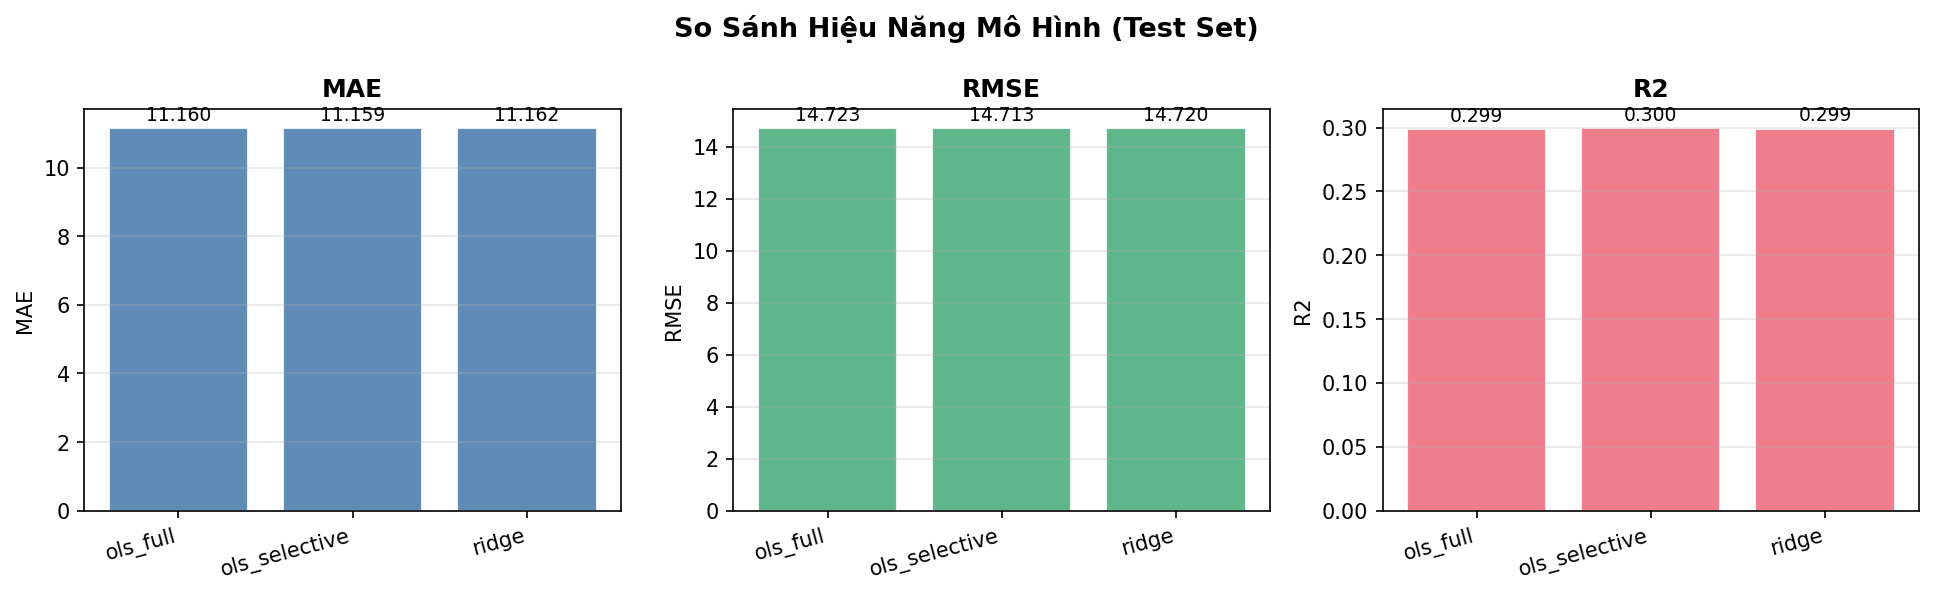
\includegraphics[width=\textwidth]{images/fig_model_comparison.png}
  \caption{Đồ thị so sánh các chỉ số lỗi trên tập Test.}
  \label{fig:model_comp_p2}
\end{minipage}
\end{figure}

\subsection{Phân tích phần dư mô hình tốt nhất}
Nhóm tiến hành phân tích phần dư chuẩn hóa của mô hình tối ưu nhất để kiểm chứng các giả thiết Gauss-Markov trên dữ liệu thực như thể hiện trong Hình \ref{fig:residual_analysis_p2}. 

\begin{figure}[H]
\centering
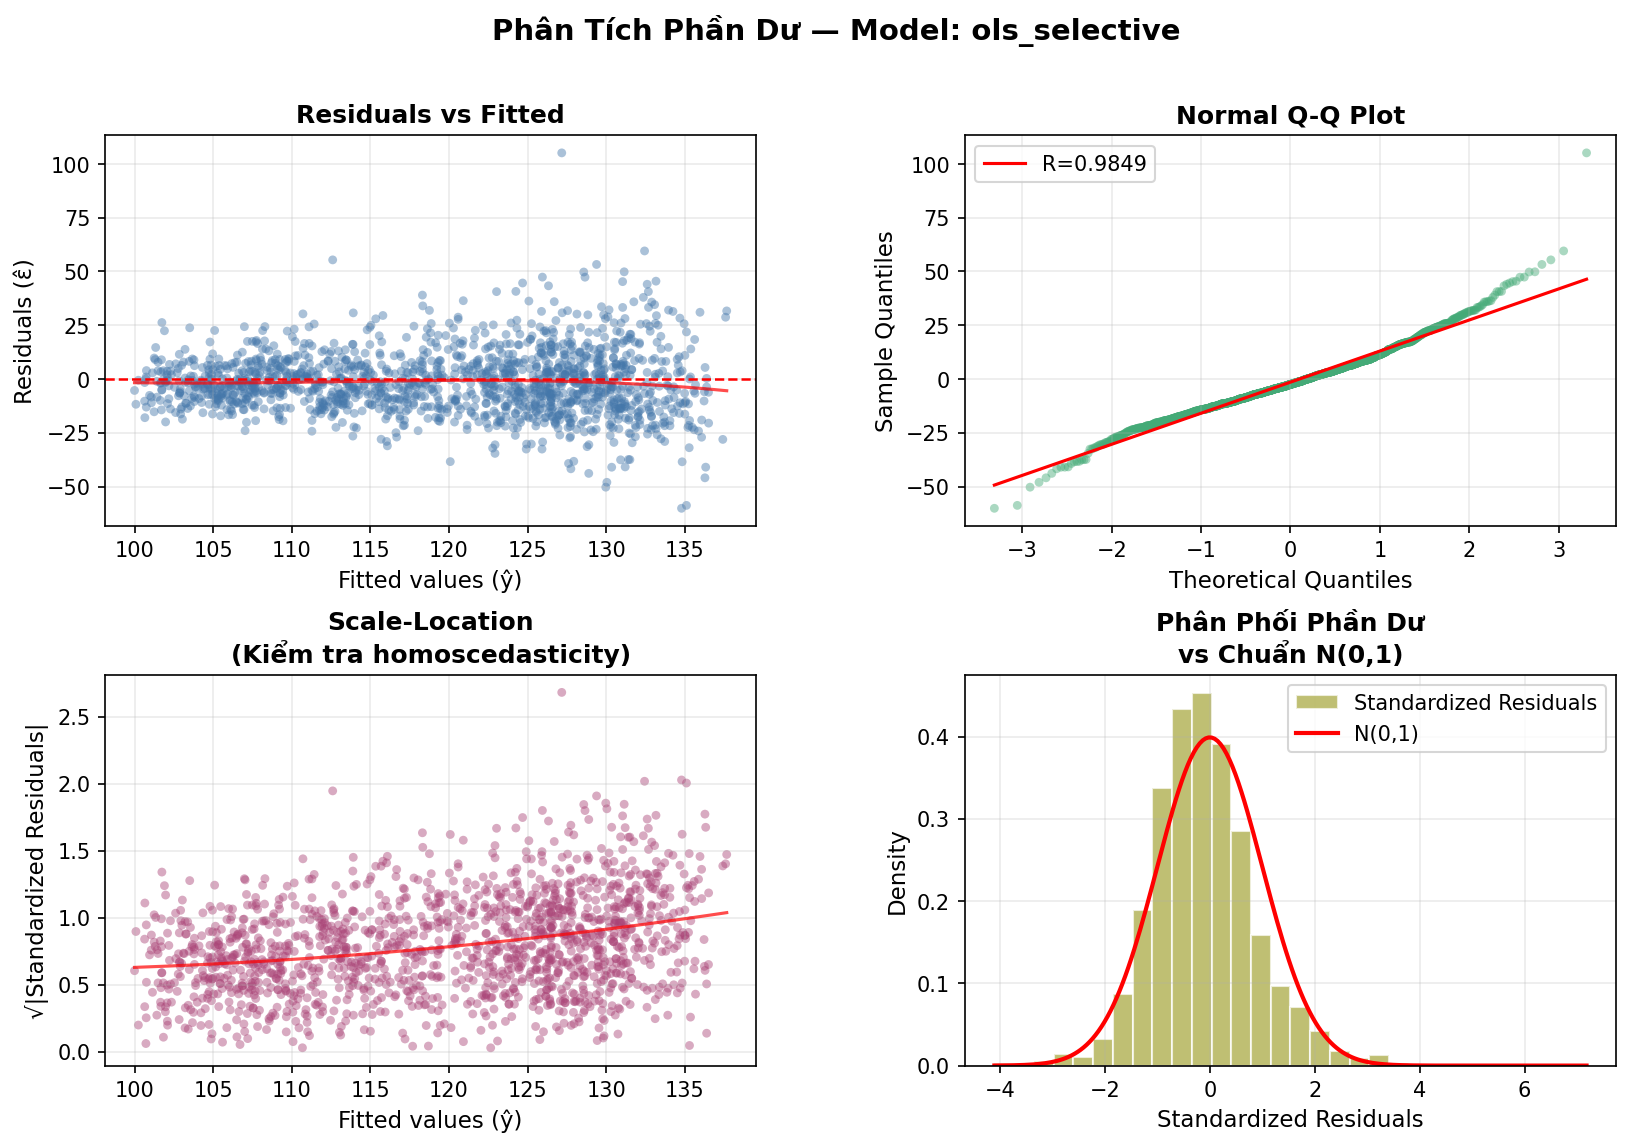
\includegraphics[width=0.75\textwidth]{images/fig_residual_analysis.png}
\caption{Bốn biểu đồ chẩn đoán phần dư của mô hình OLS chọn lọc tối ưu nhất.}
\label{fig:residual_analysis_p2}
\end{figure}

Biểu đồ Residuals vs Fitted cho thấy các điểm phần dư phân tán ngẫu nhiên đồng đều xung quanh đường chuẩn $0$ không xuất hiện cấu trúc phi tuyến, cho thấy giả thiết tuyến tính được đáp ứng tốt. Trên biểu đồ Normal Q-Q, các quan sát nằm bám sát đường phân giác $45^\circ$ khẳng định sai số tuân theo phân phối chuẩn, với hiện tượng lệch nhẹ ở các phần đuôi do biến động sinh học thực tế. Cuối cùng, đường xu hướng nằm ngang ổn định trên biểu đồ Scale-Location chứng tỏ phương sai của phần dư không đổi, thỏa mãn giả thiết đồng phương sai.

\subsection{Tầm quan trọng đặc trưng}
Tầm quan trọng của các đặc trưng được đánh giá dựa trên độ lớn của các hệ số hồi quy chuẩn hóa Z-score từ mô hình nhằm loại bỏ sự khác biệt về thang đo vật lý như mô tả trong Hình \ref{fig:feat_importance_p2}.

\begin{figure}[H]
\centering
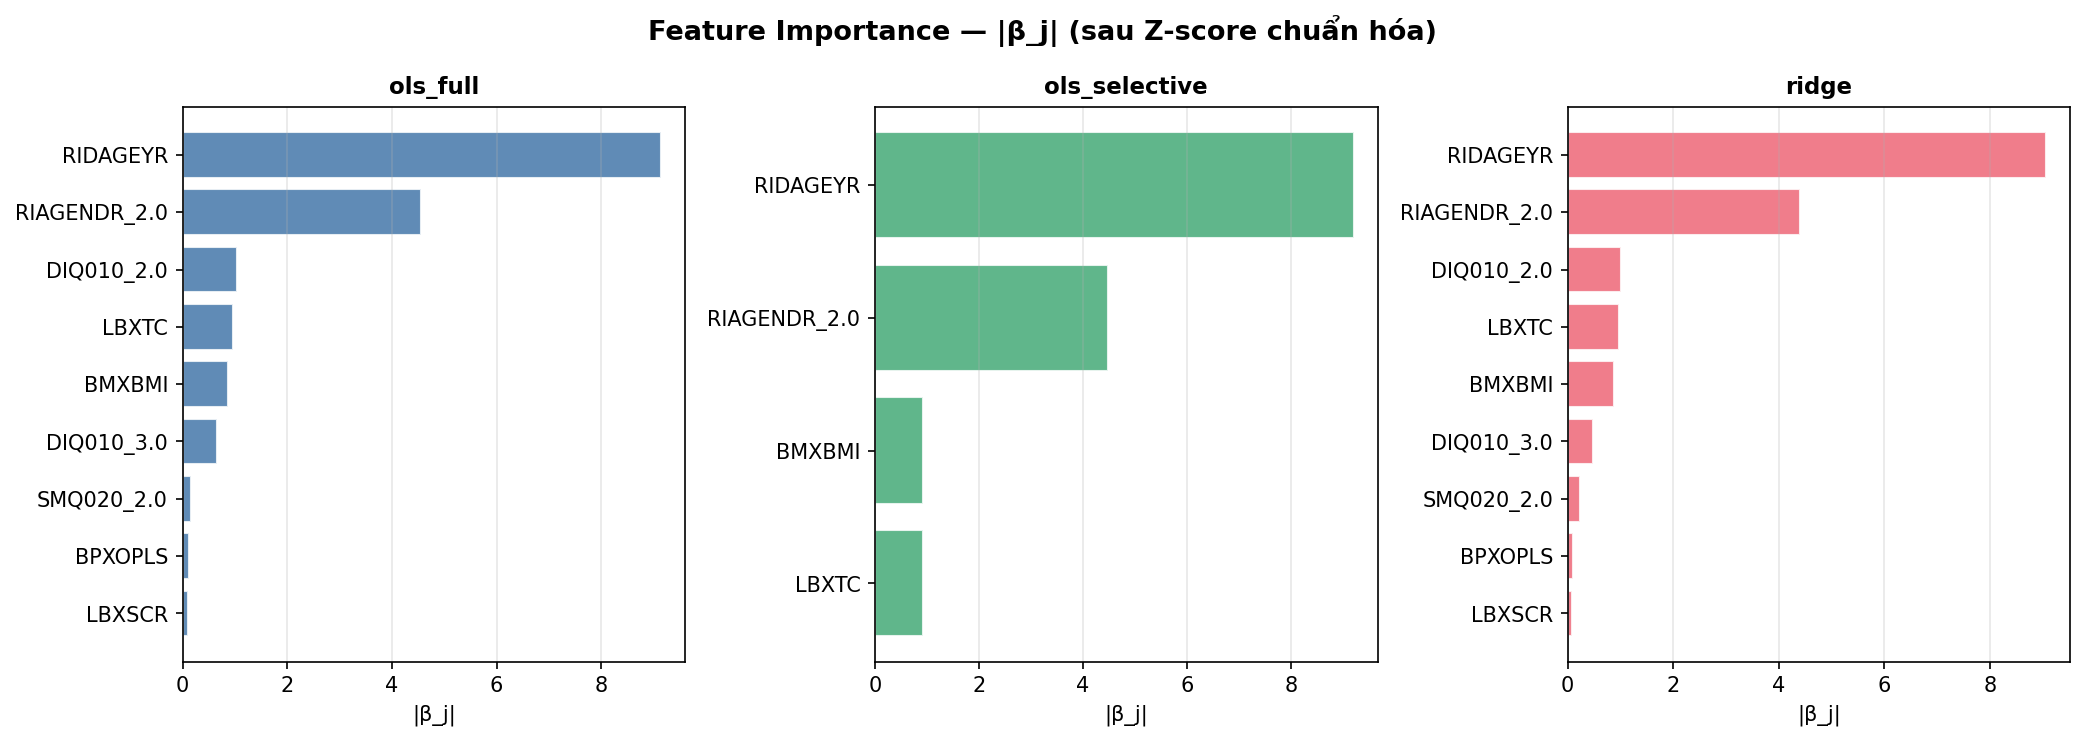
\includegraphics[width=0.6\textwidth]{images/fig_feature_importance.png}
\caption{Độ quan trọng đặc trưng của các mô hình.}
\label{fig:feat_importance_p2}
\end{figure}

Tuổi có hệ số dương lớn nhất, phù hợp với cơ chế xơ cứng thành mạch theo tuổi. BMI có tương quan thuận đáng kể do béo phì làm tăng kháng lực mạch ngoại vi. Cholesterol toàn phần có hệ số dương nhỏ hơn, liên quan đến tích tụ xơ vữa. Giới tính nữ có hệ số âm, nhất quán với tác dụng bảo vệ tim mạch của estrogen trước tuổi mãn kinh.

\subsection{Hồi quy Ridge nhân (Kernel Ridge Regression)}
Để bắt được các tương tác phi tuyến giữa các đặc trưng, nhóm cài đặt Kernel Ridge Regression (KRR) với nhân Gaussian (RBF) từ đầu. Thay vì học trực tiếp $\boldsymbol{\beta}$, KRR biểu diễn nghiệm qua vector hệ số $\boldsymbol{\alpha} \in \mathbb{R}^{n_{\text{train}}}$:
\begin{equation}
\boldsymbol{\alpha} = (\mathbf{K} + \lambda \mathbf{I})^{-1} \mathbf{y}
\end{equation}
trong đó ma trận Gram $\mathbf{K} \in \mathbb{R}^{n \times n}$ có phần tử $\mathbf{K}_{ij} = \exp\!\left(-\dfrac{\|\mathbf{x}_i - \mathbf{x}_j\|^2}{2\ell^2}\right)$. Giá trị dự đoán cho một điểm mới $\mathbf{x}^*$ được tính bằng:
\begin{equation}
\hat{y}(\mathbf{x}^*) = \mathbf{k}(\mathbf{x}^*)^T \boldsymbol{\alpha} = \mathbf{k}(\mathbf{x}^*)^T (\mathbf{K} + \lambda \mathbf{I})^{-1} \mathbf{y}
\end{equation}
với $\mathbf{k}(\mathbf{x}^*)_i = \exp\!\left(-\dfrac{\|\mathbf{x}^* - \mathbf{x}_i\|^2}{2\ell^2}\right)$ là vector kernel giữa điểm mới và toàn bộ tập Train. Do nghịch đảo ma trận $\mathbf{K}$ có chi phí $O(n^3)$, grid search tối ưu $(\lambda^*, \ell^*)$ qua 5-fold CV được thực hiện trên tập con 800 mẫu. Lưới tham số: $\lambda \in [10^{-1}, 10^3]$ và $\ell \in [10^{-1}, 10^1]$.

Kết quả tối ưu xác định bộ tham số tốt nhất là $\lambda^* = 0.1$ và $\ell^* = 10.0$. So sánh hiệu năng của Kernel Ridge trên tập Test được trình bày trong Bảng \ref{tab:krr_comparison}.

\begin{table}[H]
\centering
\caption{So sánh hiệu năng của mô hình phi tuyến Kernel Ridge với OLS đầy đủ}
\label{tab:krr_comparison}
\small
\begin{tabular}{lccc}
\toprule
\textbf{Mô hình hồi quy} & \textbf{MAE (mmHg)} & \textbf{RMSE (mmHg)} & \textbf{R²} \\
\midrule
OLS (Full) & 11.1602 & 14.7232 & 0.2988 \\
Kernel Ridge ($\lambda^*=0.1, \ell^*=10.0$) & 11.0830 & 14.8792 & 0.2839 \\
\bottomrule
\end{tabular}
\end{table}

Mô hình Kernel Ridge Regression đạt sai số tuyệt đối trung bình MAE = 11.0830 mmHg, cải thiện đáng kể so với OLS ($11.1602$ mmHg). Điều này chứng minh rằng việc ánh xạ dữ liệu phi tuyến giúp biểu diễn các đặc trưng sinh học cục bộ chính xác hơn, dù chỉ số RMSE có xu hướng nhạy cảm hơn với nhiễu lớn trong dữ liệu y tế thực tế.

\begin{figure}[H]
\centering
\begin{minipage}{0.48\textwidth}
  \centering
  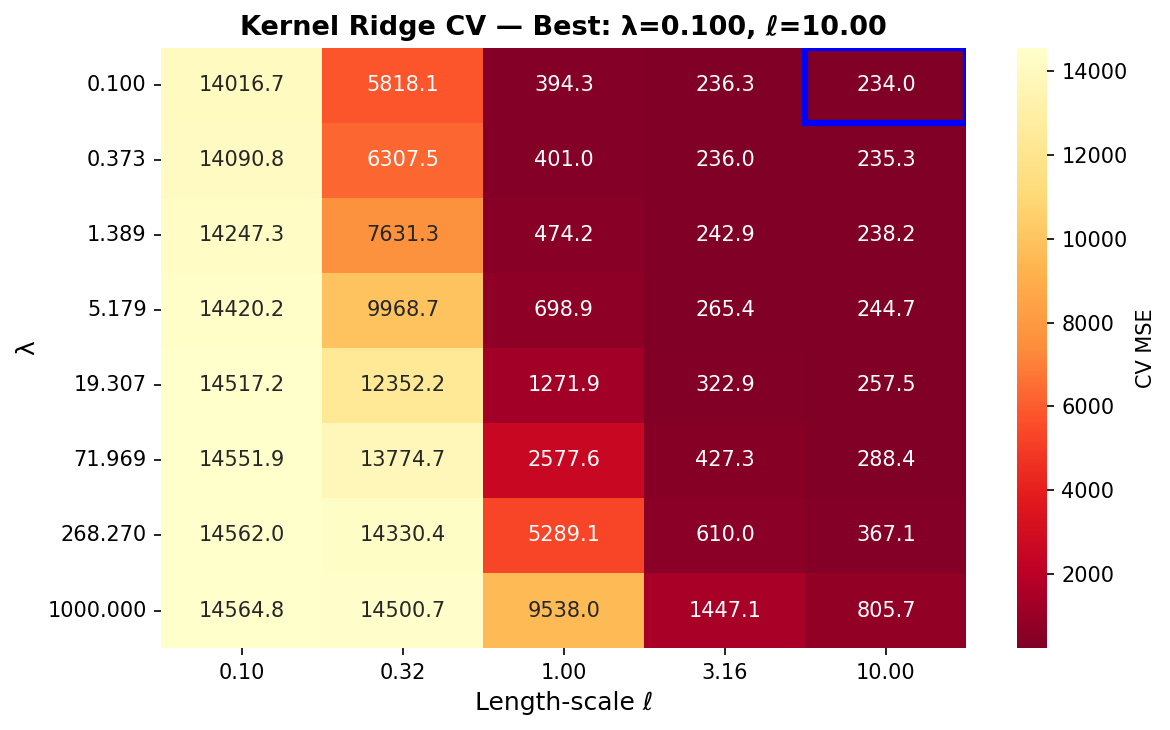
\includegraphics[width=\textwidth]{images/fig_kernel_cv_heatmap.png}
  \caption{Heatmap CV MSE trên lưới tham số 2D của KRR.}
  \label{fig:krr_heatmap}
\end{minipage}
\hfill
\begin{minipage}{0.48\textwidth}
  \centering
  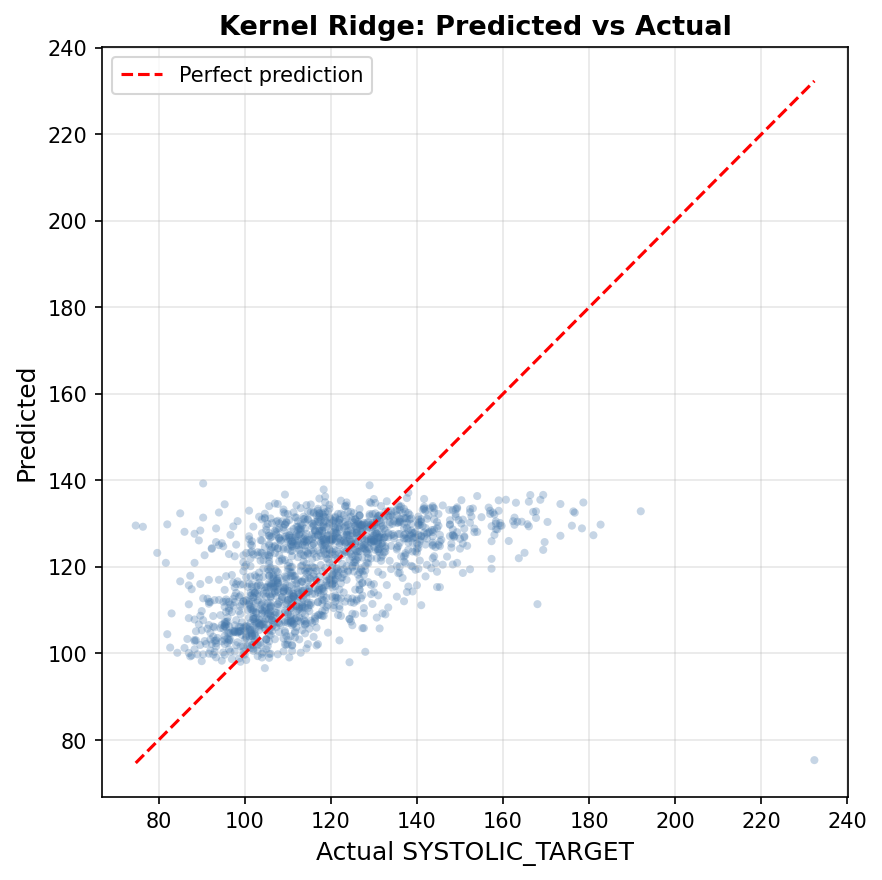
\includegraphics[width=\textwidth]{images/fig_kernel_predicted_vs_actual.png}
  \caption{Đồ thị phân tán Predicted vs Actual trên tập Test.}
  \label{fig:krr_pred_actual}
\end{minipage}
\end{figure}

\subsection{Tổng kết thực nghiệm}
Phần 2 xây dựng \texttt{DataPipeline} khép kín với KNN imputer tự cài đặt, đảm bảo không rò rỉ dữ liệu từ tập kiểm thử. Trên tập kiểm thử 1,503 mẫu, OLS Selective với 4 đặc trưng đạt RMSE = 14.71 mmHg và $\bar{R}^2 = 0.298$ — tốt hơn cả OLS đầy đủ lẫn Ridge, cho thấy chọn lọc đặc trưng hiệu quả hơn là thêm biến. Kernel Ridge Regression cải thiện MAE (11.08 so với 11.16 mmHg) nhưng RMSE cao hơn, cho thấy mô hình phi tuyến bắt được tín hiệu cục bộ nhưng nhạy hơn với outlier. Hướng mở rộng tự nhiên là hồi quy Bayesian, cho phép ước lượng khoảng tin cậy của dự đoán thay vì chỉ cho ra điểm.

% --------
\section{Kết luận}

\subsection{Nhận xét về mặt y khoa}

Sai số dự đoán RMSE $\approx 14.7$ mmHg cần được đặt trong ngữ cảnh lâm sàng. Theo tiêu chuẩn JNC 8~\cite{jnc8} và ACC/AHA 2017~\cite{aha2017}, ngưỡng phân loại tăng huyết áp giai đoạn 1 là SBP $\geq 130$ mmHg. Một sai số $\pm 14.7$ mmHg đủ để nhầm lẫn giữa các nhóm phân loại kề nhau (bình thường, tiền tăng huyết áp, giai đoạn 1), do đó mô hình không đủ độ chính xác để thay thế đo lâm sàng trực tiếp. Tuy nhiên, mục tiêu phù hợp hơn là sàng lọc nguy cơ trên quy mô dân số: ước lượng phân phối SBP trong cộng đồng và xác định nhóm có nguy cơ cao cần theo dõi, thay vì chẩn đoán cá thể.

Bốn yếu tố được mô hình chọn lọc (tuổi, BMI, cholesterol toàn phần, giới tính) đều nằm trong danh sách yếu tố nguy cơ tim mạch của WHO và AHA, và đều là các chỉ số có thể thu thập mà không cần thiết bị chuyên dụng. Điều này làm tăng tính ứng dụng của mô hình ở các cơ sở y tế tuyến cơ sở hoặc trong các khảo sát sức khỏe cộng đồng quy mô lớn, nơi đo huyết áp trực tiếp cho toàn bộ đối tượng là không khả thi.

Một hạn chế quan trọng từ góc độ y khoa là bộ dữ liệu NHANES có thiết kế cắt ngang: mỗi cá thể chỉ được đo một lần tại một thời điểm. Mô hình học được mối tương quan thống kê giữa các biến số, không phải quan hệ nhân quả theo thời gian. Do đó, các hệ số hồi quy không được diễn giải trực tiếp là ``tăng BMI thêm 1 đơn vị \emph{gây ra} tăng huyết áp $x$ mmHg'' mà chỉ là tương quan quan sát được trong quần thể tại thời điểm khảo sát.

\subsection{Hạn chế và hướng mở rộng}

Hạn chế chính của mô hình hiện tại là giả thiết tuyến tính — tác động của BMI lên huyết áp có thể khác nhau giữa các nhóm tuổi, và mô hình tuyến tính không nắm bắt được tương tác này. Bên cạnh đó, tỷ lệ khuyết thiếu cao ở cholesterol (37.8\%) và creatinine (36.5\%) đòi hỏi phải điền khuyết, làm tăng phương sai ước lượng.

Hai hướng mở rộng có giá trị thực tế nhất: (1) \textbf{Hồi quy Bayesian} — cho phép ước lượng phân phối hậu nghiệm của $\boldsymbol{\beta}$, từ đó báo cáo khoảng tin cậy dự đoán thay vì chỉ một giá trị điểm, quan trọng hơn với quyết định lâm sàng; (2) \textbf{Tích hợp thêm đặc trưng} như chỉ số creatinine (chức năng thận), tiền sử dùng thuốc hạ áp, và các biến tương tác (tuổi $\times$ BMI) để cải thiện $R^2$ mà không làm mất tính giải thích được của mô hình.

% --------
\section{Tài liệu tham khảo}

\begin{thebibliography}{9}

\bibitem{nhanes2023}
Centers for Disease Control and Prevention (CDC). \textit{National Health and Nutrition Examination Survey (NHANES) 2021--2023 Data Files}. U.S. Department of Health and Human Services, 2023. \url{https://www.cdc.gov/nchs/nhanes/}

\bibitem{strang2023}
Gilbert Strang. \textit{Introduction to Linear Algebra}, 6th ed. Wellesley-Cambridge Press, 2023.

\bibitem{hastie2021}
Gareth James, Daniela Witten, Trevor Hastie \& Robert Tibshirani. \textit{An Introduction to Statistical Learning}, 2nd ed. Springer, 2021.

\bibitem{hastie2009}
Trevor Hastie, Robert Tibshirani \& Jerome Friedman. \textit{The Elements of Statistical Learning}, 2nd ed. Springer, 2009.

\bibitem{bishop2006}
Christopher M. Bishop. \textit{Pattern Recognition and Machine Learning}. Springer, 2006.

\bibitem{murphy2022}
Kevin P. Murphy. \textit{Probabilistic Machine Learning: An Introduction}. MIT Press, 2022.

\bibitem{jnc8}
James, P.~A. et al. 2014 Evidence-Based Guideline for the Management of
High Blood Pressure in Adults: Report From the Panel Members Appointed to
the Eighth Joint National Committee (JNC~8). \textit{JAMA}, 311(5):507--520, 2014.

\bibitem{aha2017}
Whelton, P.~K. et al. 2017 ACC/AHA Guideline for the Prevention, Detection,
Evaluation, and Management of High Blood Pressure in Adults.
\textit{Journal of the American College of Cardiology}, 71(19):e127--e248, 2018.

\end{thebibliography}


\end{document}